\documentclass[12pt]{article}
\usepackage{ctex}
\usepackage[english]{babel}
\usepackage{blindtext}
\usepackage{nameref}
\usepackage{fancyhdr}
\usepackage{amsmath,amssymb,amsthm}
\usepackage{graphicx,float}
\usepackage{physics}
\usepackage{pgfplots}
\usepackage[a4paper, total={6in, 9in}]{geometry}

\graphicspath{{../image/}}

\pagestyle{fancy}
\fancyhf{}
\fancyhf[HL]{三角函數}
\fancyhf[CF]{\thepage}

\newcommand{\innerprod}[2]{\langle{#1},{#2}\rangle}
\newcommand{\id}{\mathtt{id}}

\newtheorem{definition}{定義}
\newtheorem*{theorem}{定理}
\newtheorem*{corollary}{衍理}
\newtheorem*{lemma}{引理}
\newtheorem*{proposition}{設理}
\newtheorem*{remark}{小記}
\newtheorem*{claim}{主張}
\newtheorem*{example}{例子}
\newtheorem*{axiom}{公設}
\renewenvironment*{proof}{\textit{證明.}}{\hfill$\qed$}

\newenvironment*{sol}{\par \textbf{解}.}{\hfill$\blacksquare$}

\begin{document}
    \section*{實域拓展的三角函數}

    回顧直角三角形及三角函數:

    \begin{figure}[H]
        \centering
        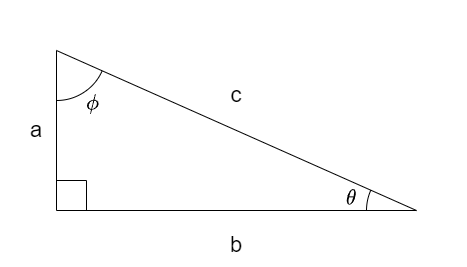
\includegraphics[scale=0.6]{triangle.png}
        \caption{邊長爲$a,b,c$的直角三角形}
    \end{figure}

    對以上直角三角形,我們定義$c$為\textbf{斜邊}。

    對於$\theta$,我們稱$a$為$\theta$的\textbf{對邊},$b$為$\theta$的\textbf{鄰邊};對於$\phi$,我們稱$b$為$\phi$的\textbf{對邊},$a$為$\phi$的\textbf{鄰邊}。

    \begin{definition}[三角函數]
        參考上述直角三角形,我們定義以下三角函數:\begin{itemize}
            \item 正弦函數(sine):$\displaystyle\sin{\theta}=\frac{a}{c}$。
            \item 餘弦函數(cosine):$\displaystyle\cos{\theta}=\frac{b}{c}$。
            \item 正切函數(tangent):$\displaystyle\tan{\theta}=\frac{a}{b}$。
            \item 正割函數(secant):$\displaystyle\sec{\theta}=\frac{c}{b}$。
            \item 餘割函數(cosecant):$\displaystyle\csc{\theta}=\frac{c}{a}$。
            \item 餘切函數(cotangent):$\displaystyle\cot{\theta}=\frac{b}{a}$。
        \end{itemize}
    \end{definition}

    \begin{remark}
        在描述三角函數的正整數次冪時,我們會寫$\sin^n{\theta}:=(\sin{\theta})^n$。但留意此寫法只適用於$n$為正整數的情況。一般而言,函數$f$的次冪以$(f)^n$記之。
    \end{remark}

    \begin{lemma}[畢氏定理]
        參考上述直角三角形,則以下等式成立:$$a^2+b^2=c^2$$
    \end{lemma}

    \begin{proposition}[恆等式]
        參考上述直角三角形,有以下恆等式:\begin{enumerate}
            \item $\sin^2{\theta}+\cos^2{\theta}=1$;
            \item $\tan{\theta}=\dfrac{\sin{\theta}}{\cos{\theta}}$;
            \item $\csc{\theta}=\dfrac{1}{\sin{\theta}}$, $\sec{\theta}=\dfrac{1}{\cos{\theta}}$, $\cot{\theta}=\dfrac{1}{\tan{\theta}}$;
            \item $\tan^2{\theta}+1=\sec^2{\theta}$, $\cot^2{\theta}+1=\csc^2{\theta}$;
            \item $\sin{\theta}=\cos{\phi}$, $\sin{\phi}=\cos{\theta}$。
        \end{enumerate}
    \end{proposition}

    \subsection*{三角函數在圓上的拓展}

    在代數幾何學中,一般考慮圓形為圓心與圓周的程差公式:考慮半徑爲$r$的圓並設圓心於原點$(0,0)$,則任何位於圓周上的點$P(x,y)$,其與圓心的距離為:$$\sqrt{x^2+y^2}=r\implies x^2+y^2=r^2$$

    若設$r=1$,我們稱其爲\textbf{單位圓}。留意圓形公式與三角恆等式$\sin^2{\theta}+\cos^2{\theta}=1$的相似性,並參考下圖:

    \begin{figure}[H]
        \centering
        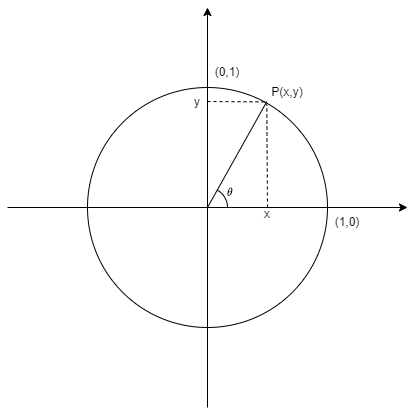
\includegraphics[scale=0.6]{circle1.png}
        \caption{半徑爲1的圓}
    \end{figure}

    由此得出,對於半徑爲1的圓,其坐標$(x,y)$亦可寫作$(\cos{\theta},\sin{\theta})$。以此爲鑒,將$\sin{\theta}$與$\cos{\theta}$的定義域從$0^\circ \leq \theta\leq 90^\circ$拓展至$0^\circ\leq \theta\leq 360^\circ$,則有以下定義:

    \begin{definition}[象限]
        按一個圓的角度$\theta$分類,給出以下名稱:\begin{itemize}
            \item 第一象限(I):$0^\circ\leq \theta\leq 90^\circ$;
            \item 第二象限(II):$90^\circ\leq \theta\leq 180^\circ$;
            \item 第三象限(III):$180^\circ\leq \theta\leq 270^\circ$;
            \item 第四象限(IV):$270^\circ\leq \theta\leq 360^\circ$。
        \end{itemize}
    \end{definition}

    第一象限為基本三角形的角度象限,至於第二、三、四象限,考慮以下圖像:

    \begin{figure}[H]
        \centering
        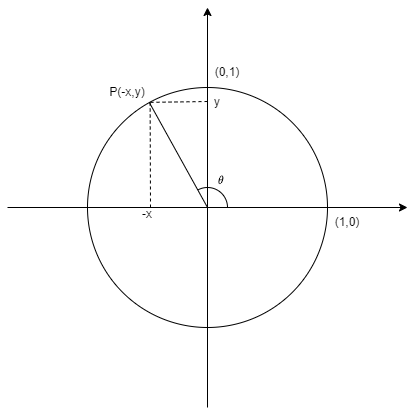
\includegraphics[scale=0.3]{circle2.png}
        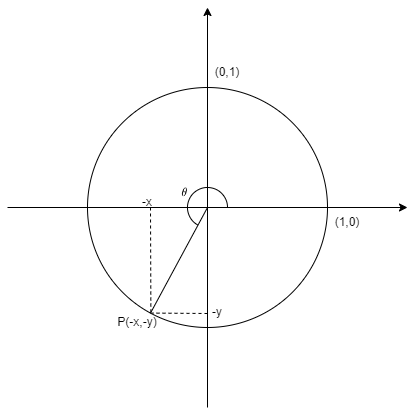
\includegraphics[scale=0.3]{circle3.png}
        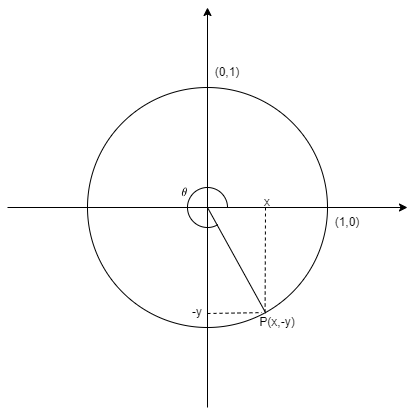
\includegraphics[scale=0.3]{circle4.png}
        \caption{第二、三、四象限的展現}
    \end{figure}

    因此,對於三角函數在圓上的拓展,我們給出以下定義:

    \begin{definition}[圓拓展三角函數]
        設$P(x,y)$為單位圓上的一點,而$\theta$為$(1,0)$展至$P$的角度,則$$x=\cos{\theta}, y=\sin{\theta}$$
    \end{definition}

    \begin{corollary}
        設$P(x,y)$為半徑$r$的圓上的一點,而$\theta$為$(r,0)$展至$P$的角度,則$$x=r\cos{\theta}, y=r\sin{\theta}$$
    \end{corollary}

    \begin{remark}
        考慮$\sin{\theta},\cos{\theta},\tan{\theta}$的值,第一象限給出所有(All)函數均爲正數,第二象限給出$\sin{\theta}$爲正數,第三象限給出$\tan{\theta}$爲正數,第四象限給出$\cos{\theta}$爲正數。故引稱C-A-S-T圖以便考慮三角函數的符號。
    \end{remark}

    至於如何求出此拓展函數的值,考慮以旋轉求出第二象限的數值:設$0^\circ\leq\theta\leq 90^\circ$,則$90^\circ\leq\theta+90^\circ\leq 180^\circ$。考慮下圖:

    \begin{figure}[H]
        \centering
        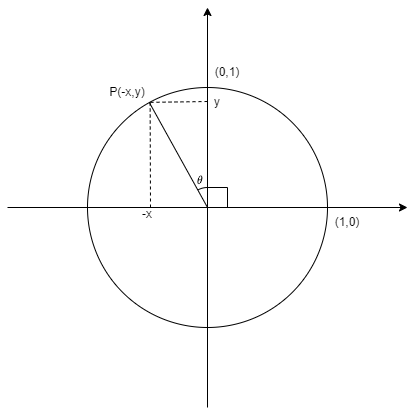
\includegraphics[scale=0.4]{circleII.png}
        $\implies$
        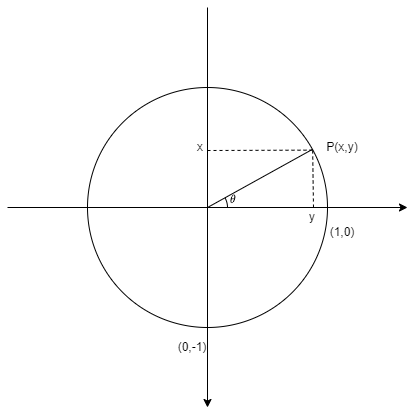
\includegraphics[scale=0.4]{circleI.png}
        \caption{以順時針方向旋轉$90^\circ$}
    \end{figure}

    留意$\sin(\theta+90^\circ)=y=\cos{\theta}$,$\cos(\theta+90^\circ)=-x=-\sin{\theta}$。因此得出\begin{align*}
        &\sin(\theta+90^\circ)=\cos{\theta},&&\cos(\theta+90^\circ)=-\sin{\theta},&&\tan(\theta+90^\circ)=-\cot{\theta}\\
        &\sin(\theta+180^\circ)=-\sin{\theta},&&\cos(\theta+180^\circ)=-\cos{\theta},&&\tan(\theta+180^\circ)=\tan{\theta}\\
        &\sin(\theta+270^\circ)=-\cos{\theta},&&\cos(\theta+270^\circ)=\sin{\theta},&&\tan(\theta+270^\circ)=-\cot{\theta}
    \end{align*}

    因圓形每$360^\circ$為一周期,故可定義:

    \begin{definition}[三角函數的周期性]
        $\sin(\theta+360^\circ)=\sin{\theta},\cos(\theta+360^\circ)=\cos{\theta}$
    \end{definition}

    \begin{theorem}
        設$\sin{\theta},\cos{\theta},\tan{\theta}$為圓拓展三角函數,$0^\circ\leq \theta\leq 90^\circ$,則:\begin{align*}
            &\sin(\pm\theta)=\pm\sin{\theta},&&\cos(\pm\theta)=\cos{\theta},&&\tan(\pm\theta)=\pm\tan{\theta}\\
            &\sin(90^\circ\pm\theta)=\cos{\theta},&&\cos(90^\circ\pm\theta)=\mp\sin{\theta},&&\tan(90^\circ\pm\theta)=\mp\cot{\theta}\\
            &\sin(180^\circ\pm\theta)=\mp\sin{\theta},&&\cos(180^\circ\pm\theta)=-\sin{\theta},&&\tan(180^\circ\pm\theta)=\pm\tan{\theta}\\
            &\sin(270^\circ\pm\theta)=-\cos{\theta},&&\cos(270^\circ\pm\theta)=\pm\sin{\theta},&&\tan(270^\circ\pm\theta)=\mp\cot{\theta}
        \end{align*}
    \end{theorem}

    \begin{corollary}
        設$\sin{\theta},\cos{\theta},\tan{\theta}$為圓拓展三角函數,$\theta$為任意角度,則:\begin{align*}
            &\sin(\pm\theta)=\pm\sin{\theta},&&\cos(\pm\theta)=\cos{\theta},&&\tan(\pm\theta)=\pm\tan{\theta}\\
            &\sin(90^\circ\pm\theta)=\cos{\theta},&&\cos(90^\circ\pm\theta)=\mp\sin{\theta},&&\tan(90^\circ\pm\theta)=\mp\cot{\theta}\\
            &\sin(180^\circ\pm\theta)=\mp\sin{\theta},&&\cos(180^\circ\pm\theta)=-\sin{\theta},&&\tan(180^\circ\pm\theta)=\pm\tan{\theta}\\
            &\sin(270^\circ\pm\theta)=-\cos{\theta},&&\cos(270^\circ\pm\theta)=\pm\sin{\theta},&&\tan(270^\circ\pm\theta)=\mp\cot{\theta}
        \end{align*}
    \end{corollary}

    \begin{definition}[弧度]
        依照圓周計算,定義\textbf{弧度}為角度對應的單位弧長路徑,並以rad爲單位(使用時可忽略單位不寫)。$\pi$對應$180^\circ$。
    \end{definition}

    \begin{corollary}
        設$\sin{\theta},\cos{\theta},\tan{\theta}$為圓拓展三角函數,$\theta$為任意角度,則:\begin{align*}
            &\sin(\pm\theta)=\pm\sin{\theta},&&\cos(\pm\theta)=\cos{\theta},&&\tan(\pm\theta)=\pm\tan{\theta}\\
            &\sin(\frac{\pi}{2}\pm\theta)=\cos{\theta},&&\cos(\frac{\pi}{2}\pm\theta)=\mp\sin{\theta},&&\tan(\frac{\pi}{2}\pm\theta)=\mp\cot{\theta}\\
            &\sin(\pi\pm\theta)=\mp\sin{\theta},&&\cos(\pi\pm\theta)=-\sin{\theta},&&\tan(\pi\pm\theta)=\pm\tan{\theta}\\
            &\sin(\frac{3\pi}{2}\pm\theta)=-\cos{\theta},&&\cos(\frac{3\pi}{2}\pm\theta)=\pm\sin{\theta},&&\tan(\frac{3\pi}{2}\pm\theta)=\mp\cot{\theta}
        \end{align*}
    \end{corollary}

    \subsection*{逆三角函數}

    考慮三角函數作爲函數的可逆性並不理想(不符合單射性),故對於逆三角函數的討論,雖稱其爲逆函數,卻視之為逆映射。

    \begin{definition}[三角函數的逆函數]
        對於逆三角函數,給出以下定義:\begin{align*}
            &\arcsin:\{-1\leq x\leq 1\}\to\mathbb{R},&&x\mapsto\{\theta\in\mathbb{R}:\sin{\theta}=x\}\\
            &\arccos:\{-1\leq x\leq 1\}\to\mathbb{R},&&x\mapsto\{\theta\in\mathbb{R}:\cos{\theta}=x\}\\
            &\arctan:\mathbb{R}\to\mathbb{R},&&x\mapsto\{\theta\in\mathbb{R}:\tan{\theta}=x\}
        \end{align*}
        同理,對於另外三個三角函數:\begin{align*}
            &\arcsec:\{-1\leq x\leq 1\}\to\mathbb{R},&&x\mapsto\{\theta\in\mathbb{R}:\sec{\theta}=x\}\\
            &\arccsc:\{-1\leq x\leq 1\}\to\mathbb{R},&&x\mapsto\{\theta\in\mathbb{R}:\csc{\theta}=x\}\\
            &\arccot:\mathbb{R}\to\mathbb{R},&&x\mapsto\{\theta\in\mathbb{R}:\cot{\theta}=x\}
        \end{align*}
    \end{definition}

    \begin{remark}
        留意前綴`arc',其意義為`求弧度'。因此意義上與求角度是一樣的,惟需注意的是因應三角函數的周期性,符合條件的結果有無窮多項,因此定義以數集表示。通常所求角度在$0$至$2\pi$之間,對應結果有兩項。若限於$0$至$\pi/2$之間,則可視爲逆函數,亦是常規解釋,分別記爲$\sin^{-1},\cos^{-1},\tan^{-1},\sec^{-1},\csc^{-1},\cot^{-1}$。
    \end{remark}

    \begin{proposition}
        對於$x\in\mathbb{R}$,\begin{align*}
            &\arcsin(\sin{x})=\{2n\pi+x, (2n+1)\pi-x:n\textrm{為整數}\}\\
            &\arccos(\cos{x})=\{2n\pi\pm x:n\textrm{為整數}\}\\
            &\arctan(\tan{x})=\{n\pi+x:n\textrm{為整數}\}
        \end{align*}
    \end{proposition}

    \section*{三角函數的和積互化}

    目前已知特殊角度的加減可簡化爲單一角度的算式,如此衍伸問題:對於任意角度$\alpha,\beta$,若寫$\sin(\alpha+\beta),\cos(\alpha+\beta),\tan(\alpha+\beta)$,能否將之簡化爲$\alpha$與$\beta$的三角函數算式呢?即是否有函數$f,g,h$使得\begin{align*}
        \sin(\alpha+\beta)&=f(\sin{\alpha},\sin{\beta},\cos{\alpha},\cos{\beta},\tan{\alpha},\tan{\beta})\\
        \cos(\alpha+\beta)&=g(\sin{\alpha},\sin{\beta},\cos{\alpha},\cos{\beta},\tan{\alpha},\tan{\beta})\\
        \tan(\alpha+\beta)&=h(\sin{\alpha},\sin{\beta},\cos{\alpha},\cos{\beta},\tan{\alpha},\tan{\beta})
    \end{align*}

    從$\sin(\alpha+\beta)$入手,考慮以下扇形

    \begin{figure}[H]
        \centering
        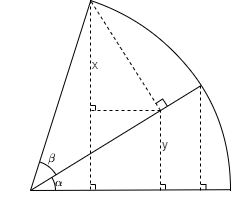
\includegraphics[scale=0.8]{ab.png}
    \end{figure}

    如上圖所示,$\sin(\alpha+\beta)=x+y$。又見$$x=\sin{\beta}\cos{\alpha}, y=\cos{\beta}\sin{\alpha}$$則$\sin(\alpha+\beta)=\sin{\alpha}\cos{\beta}+\sin{\beta}\cos{\alpha}$。

    現求得$\sin(\alpha+\beta)$的變化,則可通過代入求得其餘變化:\begin{align*}
        \sin(\alpha-\beta)&=\sin(\alpha+(-\beta))=\sin{\alpha}\cos(-\beta)+\sin(-\beta)\cos{\alpha}\\&=\sin{\alpha}\cos{\beta}-\sin{\beta}\cos{\alpha}\\
        \cos(\alpha+\beta)&=\sin(\frac{\pi}{2}-(\alpha+\beta))=\sin(\frac{\pi}{2}-\alpha)\cos(-\beta)+\sin(-\beta)\cos(\frac{\pi}{2}-\alpha)\\&=\cos{\alpha}\cos{\beta}-\sin{\alpha}\sin{\beta}\\
        \cos(\alpha-\beta)&=\cos(\alpha+(-\beta))=\cos{\alpha}\cos(-\beta)-\sin{\alpha}\sin(-\beta)\\&=\cos{\alpha}\cos{\beta}+\sin{\alpha}\sin{\beta}\\
        \tan(\alpha+\beta)&=\frac{\sin(\alpha+\beta)}{\cos(\alpha+\beta)}=\frac{\sin{\alpha}\cos{\beta}+\sin{\beta}\cos{\alpha}}{\cos{\alpha}\cos{\beta}-\sin{\alpha}\sin{\beta}}\\&=\frac{\frac{\sin{\alpha}}{\cos{\alpha}}+\frac{\sin{\beta}}{\cos{\beta}}}{1-\frac{\sin{\alpha}}{\cos{\alpha}}\frac{\sin{\beta}}{\cos{\beta}}}=\frac{\tan{\alpha}+\tan{\beta}}{1-\tan{\alpha}\tan{\beta}}\\
        \tan(\alpha-\beta)&=\frac{\tan{\alpha}+\tan(-\beta)}{1-\tan{\alpha}\tan(-\beta)}\\
        &=\frac{\tan{\alpha}-\tan{\beta}}{1+\tan{\alpha}\tan{\beta}}
    \end{align*}

    \begin{theorem}
        設$\alpha,\beta$為弧度角,則\begin{align*}
            &\sin(\alpha\pm\beta)=\sin{\alpha}\cos{\beta}\pm\sin{\beta}\cos{\alpha}\\
            &\cos(\alpha\pm\beta)=\cos{\alpha}\cos{\beta}\mp\sin{\alpha}\sin{\beta}\\
            &\tan(\alpha\pm\beta)=\frac{\tan{\alpha}\pm\tan{\beta}}{1\mp\tan{\alpha}\tan{\beta}}
        \end{align*}
    \end{theorem}

    由此,可逆推算出以下設理:

    \begin{proposition}
        設$\alpha,\beta$為弧度角,則\begin{align*}
            &\sin{\alpha}\cos{\beta}=\frac{1}{2}[\sin(\alpha-\beta)+\sin(\alpha+\beta)]\\
            &\sin{\alpha}\sin{\beta}=\frac{1}{2}[\cos(\alpha-\beta)-\cos(\alpha+\beta)]\\
            &\cos{\alpha}\cos{\beta}=\frac{1}{2}[\cos(\alpha-\beta)+\cos(\alpha+\beta)]
        \end{align*}
    \end{proposition}

    \begin{corollary}
        設$\alpha,\beta$為弧度角,則\begin{align*}
            &\sin{\alpha}\pm\sin{\beta}=2\sin{\frac{\beta\pm\alpha}{2}}\cos{\frac{\beta\mp\alpha}{2}}\\
            &\cos{\alpha}+\cos{\beta}=2\cos{\frac{\beta+\alpha}{2}}\cos{\frac{\beta-\alpha}{2}}\\
            &\cos{\alpha}-\cos{\beta}=2\sin{\frac{\beta+\alpha}{2}}\sin{\frac{\beta-\alpha}{2}}\\
        \end{align*}
    \end{corollary}

    \subsection*{兩倍角公式}

    從以上和積互化公式可見,若$\alpha=\beta$,則可視爲\textbf{兩倍角公式}:

    \begin{theorem}
        設$x$為弧度角,則\begin{align*}
            &\sin(2x)=2\sin{x}\cos{x}\\
            &\cos(2x)=\cos^2{x}-\sin^2{x}\\
            &\tan(2x)=\frac{2\tan{x}}{1-\tan^2{x}}
        \end{align*}
    \end{theorem}

    留意$\cos(2x)=\cos^2{x}-\sin^2{x}$可化為\begin{align*}
        \cos^2{x}-\sin^2{x}&=(1-\sin^2{x})-\sin^2{x}\\
        &=1-2\sin^2{x}
    \end{align*}
    或\begin{align*}
        \cos^2{x}-\sin^2{x}&=\cos^2{x}-(1-\cos^2{x})\\
        &=2\cos^2{x}-1
    \end{align*}

    故當$0<x<\pi$時,$$\sin{x}=\sqrt{\frac{1-\cos(2x)}{2}}\implies\sin{\frac{t}{2}}=\sqrt{\frac{1-\cos{t}}{2}}$$
    當$0<x<\frac{\pi}{2}$時,$$\cos{x}=\sqrt{\frac{1+\cos(2x)}{2}}\implies\cos{\frac{t}{2}}=\sqrt{\frac{1+\cos{t}}{2}}$$
    當$\frac{\pi}{2}<x<\pi$時,$$\cos{x}=-\sqrt{\frac{1+\cos(2x)}{2}}\implies\cos{\frac{t}{2}}=-\sqrt{\frac{1+\cos{t}}{2}}$$
    其中$t=2x$。此算式稱爲\textbf{半倍角公式}。

    同時考慮$t=\tan{\frac{x}{2}}$,則對於所有三角函數,均可以$t$表示。以$\sin{x}$爲例:\begin{align*}
        \sin{x}&=2\sin{\frac{x}{2}}\cos{\frac{x}{2}}\\
        &=\frac{2\tan{\frac{x}{2}}}{\sec^2{\frac{x}{2}}}\\
        &=\frac{2t}{1+t^2}
    \end{align*}

    對此,以下定理成立:

    \begin{theorem}
        設$x\in\mathbb{R}$,若$t=\tan{\frac{x}{2}}$,則\begin{align*}
            &\sin{x}=\frac{2t}{1+t^2},&&\cos{x}=\frac{1-t^2}{1+t^2},&&\tan{x}=\frac{2t}{1-t^2}
        \end{align*}
    \end{theorem}

    \subsection*{三倍角公式}

    \begin{theorem}
        設$x\in\mathbb{R}$,則\begin{align*}
            &\sin(3x)=3\sin{x}-4\sin^3{x}\\
            &\cos(3x)=4\cos^3{x}-3\cos{x}\\
            &\tan(3x)=\frac{3\tan{x}-\tan^3{x}}{1-3\tan^2{x}}
        \end{align*}
    \end{theorem}

    \begin{proof}
        重複運用兩倍角公式以推導出$\sin(3x)$和$\cos(3x)$的算式,並運用$\tan(3x)=\dfrac{\sin(3x)}{\cos(3x)}$推導結果。
    \end{proof}

    \subsection*{輔助角}

    回顧和積互化公式,大部分三角學算式都能化作$\sin$與$\cos$的組合,如此便能讓大部分等式迎刃而解。但亦有例外:$$2\sin{x}+3\cos{x}=4$$

    對於以上等式,我們無法直接套用任何一條三角形公式以求得答案。如此便需要額外技巧,稱爲\textbf{輔助角}。在運用輔助角時需要一定條件,考慮通用式:$$a\sin{x}+b\cos{x}=c$$其中$a,b,c\in\mathbb{R}$。考慮左邊算式與$\sin(x+y)$的展開式的相似性,便作以下猜想:

    \begin{claim}
        設存在$r$與$\alpha$使得以下等式成立:$$r\sin(x+\alpha)=a\sin{x}+b\cos{x}$$且$r\geq |c|$,則$a\sin{x}+b\cos{x}=c$可解。
    \end{claim}

    \begin{proof}
        直接計算即可。若\begin{align*}
            r\sin(x+\alpha)&=a\sin{x}+b\cos{x}
        \end{align*}
        則\begin{align*}
            r\sin{x}\cos{\alpha}+r\cos{x}\sin{\alpha}&=a\sin{x}+b\cos{x}\\
            \implies&\begin{cases}
                r\cos{\alpha}=a\\
                r\sin{\alpha}=b
            \end{cases}\\
            \implies&\begin{cases}
                r=\sqrt{a^2+b^2}\\
                \alpha=\tan^{-1}(\frac{b}{a})
            \end{cases}
        \end{align*}

        同時$$r\sin(x+\alpha)=c\implies \sin(x+\alpha)=\frac{c}{r}$$
        由於$\sin{x}$的值域介乎$-1$與$1$之間,故$|c|/r\leq 1\implies |c|\leq r$時等式可解。
    \end{proof}

    \begin{theorem}
        設$a,b,c$為常數,$x\in\mathbb{R}$。當$a^2+b^2\geq c^2$時,則$a\sin{x}+b\cos{x}=c$的解為$$x=\sin^{-1}(\frac{c}{\sqrt{a^2+b^2}})-\tan^{-1}(\frac{b}{a})$$
    \end{theorem}

    \section*{複域幾何}

    回顧中四對於複數的教學:對於任意複數$z\in\mathbb{C}$,均可寫$$z=x+yi$$其中$x,y\in\mathbb{R}$,$i^2=-1$。此表達式稱爲\textbf{標準式}(或稱\textbf{笛卡爾式}),因爲對於任何複數而言,此表達式都是獨特的,而且可輕易區分\textbf{實部}和\textbf{複部}:\begin{itemize}
        \item 實部:記$\Re{z}=x$;
        \item 複部:記$\Im{z}=y$;
    \end{itemize}

    對此,考慮$i$並非實數,則可假設$i$為與實數綫垂直的方向。由此引用\textbf{阿根圖}:

    \begin{figure}[H]
        \centering
        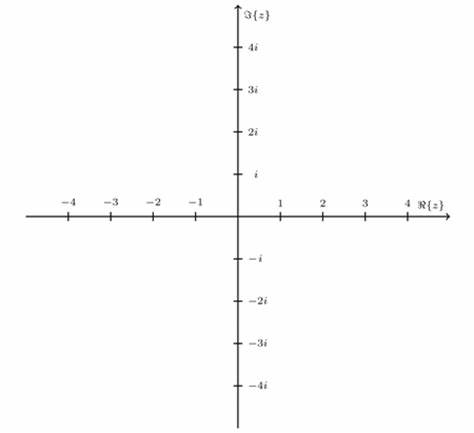
\includegraphics[scale=0.6]{argand.jpg}
    \end{figure}

    以此爲鑒,此圖考慮等價於\textbf{笛卡爾坐標圖},作y軸為$\Im{z}$的向量,x軸為$\Re{z}$的向量,則任何複數$z=x+yi\in\mathbb{C}$,都可記爲:$$x+yi\sim(x,y)$$
    並且留意到\begin{align*}
        i&=0+1i\sim(0,1)\\
        (a,b)+(c,d)\sim (a+bi)+(c+di)&=(a+c)+(b+d)i\sim(a+c,b+d)\\
        (a,b)\cdot (c,d)\sim(a+bi)(c+di)&=(ac-bd)+(ad+bc)i\sim(ac-bd,ad+bc)
    \end{align*}

    運用坐標可使我們對複數的理解更具體。現定義:

    \begin{definition}[模]
        對於$z\in\mathbb{C}$,我們稱$z$與$0$的距離為\textbf{模},並記為:$$|z|=\sqrt{(\Re{z})^2+(\Im{z})^2}$$
    \end{definition}

    \begin{definition}[模]
        對於$z\in\mathbb{C}$,定義$z$的\textbf{共軛}為:$$\overline{z}=\Re{z}-\Im{z}$$若以坐標描述,可定義爲$(x,y)\mapsto(x,-y)$,並視爲沿實數軸反射。
    \end{definition}

    \begin{proposition}
        對於任意$z\in\mathbb{C}-\{0\}$,均有$$|z|=\sqrt{z\overline{z}}$$
    \end{proposition}

    \begin{corollary}
        對於任意$z\in\mathbb{C}-\{0\}$,$z$可逆,並且$$z^{-1}=\frac{\overline{z}}{|z|^2}$$
    \end{corollary}

    \begin{remark}
        需注意$0$沒有逆元素,除非對於$\dfrac{1}{0}$有明確定義,否則不作考慮。詳細參考\textbf{擴充平面}的敘述。
    \end{remark}

    考慮笛卡爾平面與極坐標的轉換,參考

    \begin{figure}[H]
        \centering
        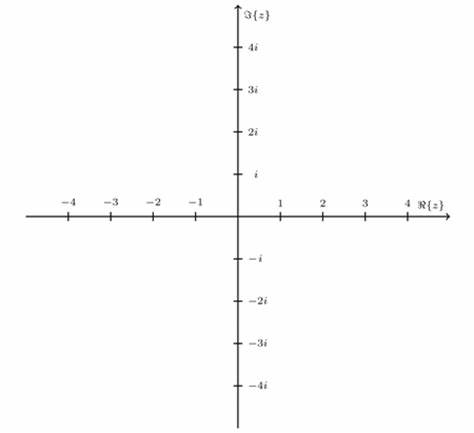
\includegraphics[scale=0.5]{argand.jpg}
        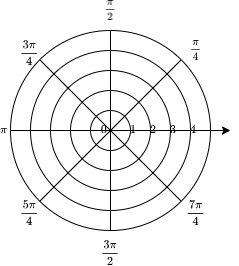
\includegraphics[scale=0.5]{polar.png}
        \caption{阿根圖與極坐標}
    \end{figure}

    坐標的對應方式如下:

    \begin{center}
        \begin{tabular}{|c|c|c|}
            \hline
            複數&笛卡爾&極坐標\\
            \hline
            0&(0,0)&(0,0)\\
            \hline
            $1$&$(1,0)$&$(1,0)$\\
            \hline
            $i$&$(0,1)$&$(1,\pi/2)$\\
            \hline
            $-1$&$(-1,0)$&$(1,\pi)$\\
            \hline
            $-i$&$(0,-1)$&$(1,3\pi/2)$\\
            \hline
        \end{tabular}
    \end{center}

    並且回憶圓形與三角函數的關係,可得以下表達式:

    \begin{theorem}
        對於任意$z\in\mathbb{C}$,均可寫作$$z=r(\cos{\theta}+i\sin{\theta})$$其中$r=|z|,\theta=\arctan{\frac{\Im{z}}{\Re{z}}}$。
    \end{theorem}

    \begin{proof}
        考慮單位圓:
        \begin{figure}[H]
            \centering
            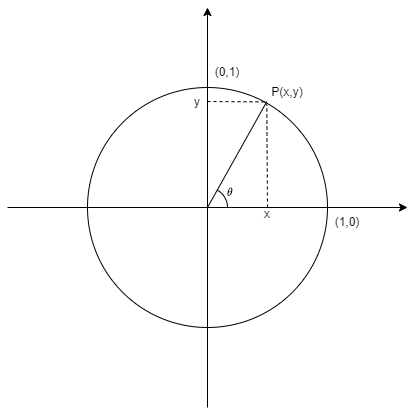
\includegraphics[scale=0.6]{circle1.png}
        \end{figure}
        並由定義3之衍理,可得$z\sim(r\cos{\theta},r\sin{\theta})\sim r\cos{\theta}+ir\sin{\theta}=r(\cos{\theta}+i\sin{\theta})$。其中\begin{align*}
            |z|&=\sqrt{(r\cos{\theta})^2+(r\sin{\theta})^2}\\
            &=\sqrt{r^2}\\
            &=r\\
            \tan{\theta}&=\frac{r\sin{\theta}}{r\cos{\theta}}=\frac{\Im{z}}{\Re{z}}\\
            \theta&=\arctan{\frac{\Im{z}}{\Re{z}}}
        \end{align*}
    \end{proof}

    \section*{棣莫弗定理與多倍角}

    對於複數加減法,我們不再多説,因爲加減法屬於非常簡單的運算。但是,對於乘除法,我們可有更深刻的瞭解,而且其中牽涉的很大程度與三角函數有關。

    \begin{theorem}[棣莫弗定理]
        設$z,w\in\mathbb{C}$,並表$z=r(\cos{\theta}+i\sin{\theta}),w=s(\cos{\phi}+i\sin{\phi})$。則$$zw=rs(\cos(\theta+\phi)+i\sin(\theta+\phi))$$
    \end{theorem}

    \begin{proof}
        通過直接計算:\begin{align*}
            zw&=r(\cos{\theta}+i\sin{\theta})s(\cos{\phi}+i\sin{\phi})\\
            &=rs(\cos{\theta}+i\sin{\theta})(\cos{\phi}+i\sin{\phi})\\
            &=rs(\cos{\theta}\cos{\phi}-\sin{\theta}\sin{\phi}+i(\cos{\theta}\sin{\phi}+\sin{\theta}\cos{\phi}))\\
            &=rs(\cos(\theta+\phi)+i\sin(\theta+\phi))
        \end{align*}
    \end{proof}

    \begin{proposition}[棣莫弗定理的推廣形式]
        設$(z_k)_{k=1}^n$為一系列複數,其中對於所有$1\leq k\leq n$,$z_k=r_k(\cos{\theta_k}+i\sin{\theta_k})$。則$$\prod_{k=1}^{n}z_k=(\prod_{k=1}^{n}r_k)[\cos(\sum_{k=1}^{n}\theta_k)+i\sin(\sum_{k=1}^{n}\theta_k)]$$
    \end{proposition}

    \begin{proof}
        運用數學歸納法。
    \end{proof}

    \begin{proposition}[乘方形式]
        對於任意$z\in\mathbb{C}$,若$z=r(\cos{\theta}+i\sin{\theta})$,則對於任何整數$n$,均有$$z^n=r^n(\cos(n\theta)+i\sin(n\theta))$$
    \end{proposition}

    \begin{proof}
        推廣形式中所有$\theta_k$相等時的結果。
    \end{proof}

    \begin{corollary}
        若考慮乘方形式中$r=1$,即模為1的複數,則$$(\cos{\theta}+i\sin{\theta})^n=\cos(n\theta)+i\sin(n\theta)$$
    \end{corollary}

    根據以上衍理,可得出多倍角的算式為\begin{align*}
        \cos(nx)&=\sum_{0\leq k\leq n/2}\cos^{n-2k}{x}\sin^{2k}{x}\\
        \sin(nx)&=\sum_{0\leq k\leq n/2}\cos^{n-2k-1}{x}\sin^{2k+1}{x}\\
    \end{align*}

    \section*{習題}
    \begin{enumerate}
        \item 試證明正弦、餘弦定理,及希羅公式:設$\triangle ABC$中$a$為$\angle A$的對邊邊長,$b$為$\angle B$的對邊邊長,$c$為$\angle C$的對邊邊長。\begin{itemize}
            \item 正弦定理:$\dfrac{\sin{A}}{a}=\dfrac{\sin{B}}{b}=\dfrac{\sin{C}}{c}$
            \item 餘弦定理:$c^2=a^2+b^2-2ab\cos{\angle C}$
            \item 希羅公式:定義$s=\dfrac{a+b+c}{2}$,$$\textrm{面積}=\sqrt{s(s-a)(s-b)(s-c)}$$
        \end{itemize}
        \item 求以下$x$的值($0\leq x \leq 2\pi$):\begin{align*}
            &\textrm{a) } \sin{x}=\dfrac{1}{2} && \textrm{b) } \cot{x}=-\dfrac{1}{3} && \textrm{c) } \cos{x}=\dfrac{3}{5} && \textrm{d) } \tan{x}=1\\
            &\textrm{e) } \cot{x}=3 && \textrm{f) } \cos{x}=-0.5 && \textrm{g) } \sin{x}=\dfrac{\sqrt{2}}{2} && \textrm{h) } \tan{x}=-2.4\\
            &\textrm{i) } \sin{x}=-0.4 && \textrm{j) } \cos{x}=-1 && \textrm{k) } \tan{x}=-\sqrt{3} && \textrm{l) } \cot{x}=\dfrac{1}{7}
        \end{align*}
        \item 簡化以下表達式:\begin{align*}
            &\textrm{a) } \frac{\sin^2{x}}{1-\cos{x}} && \textrm{b) } \frac{\sin{x}}{1+\cos{x}}+\frac{1+\cos{x}}{\sin{x}}\\
            &\textrm{c) } \frac{\tan{x}\tan{2x}}{\tan{x}-\tan{2x}} && \textrm{d) } \frac{1-\cos{2x}}{\sin{2x}}+\frac{\sin{2x}}{1+\cos{2x}}\\
            &\textrm{e) } \frac{\sin{u}+\sin{v}}{\cos{u}+\cos{v}} && \textrm{f) } \frac{\sin{x}+\sin{3x}+\sin{5x}+\sin{7x}}{\cos{x}+\cos{3x}+\cos{5x}+\cos{7x}}\\
            &\textrm{g) } \sin{x}\cot{x}+\cos{x} && \textrm{h) } \sin^2{x}(1+\cot{x})+\cos^2{x}(1+\tan{x})-1-\sin{2x}\\
            &\textrm{i) } \frac{\cos{x}-\sin{x}}{1-\tan{x}} && \textrm{j) } \frac{\cos{3x}+\cos{x}}{\cos{4x}+\cos{2x}}+\frac{\sin{3x}+\sin{x}}{\sin{4x}+\sin{2x}}\\
            &\textrm{k) } \frac{1+\cos{2x}}{1-\cos{2x}} && \textrm{l) } \frac{1}{1-\sin{x}}-\frac{\sin{x}}{1-\sin^2{x}}-\frac{1}{1+\sin{x}}\\
            &\textrm{m) } \frac{\sin{2x}}{\cos^2{x}} && \textrm{n) } \frac{\sin{x}+\sin{5x}-\sin{3x}}{\cos{x}+\cos{5x}-\cos{3x}}\\
            &\textrm{o) } \frac{1-\tan^2{x}}{\cos{2x}} && \textrm{p) } \frac{1+\cos{2x}}{1-\cos{x}}-\frac{4\cos^2{(x/2)}}{\tan^2{x}}\\
            &\textrm{q) } \frac{\sin^2{x}-1}{\cos^2{x}-1} && \textrm{r) } \frac{\sin(\pi/6+x)-\sin(\pi/6-x)}{\cos(\pi/3+x)+\cos{\pi/3-x}}\\
            &\textrm{s) } \frac{2\tan{x}}{1+\tan^2{x}} && \textrm{t) } \cos(\pi/4+x)-\cos(\pi/4-x)\\
        \end{align*}
        \item 證明以下等式:$$\sin^2(n\theta)-\sin^2(m\theta)=\sin[(n+m)\theta]\sin[(n-m)\theta]$$由此,解方程$\sin^2(3\theta)-\sin^2(2\theta)-\sin{\theta}=0$,其中$0\leq \theta\leq \pi$。
        \item \begin{enumerate}
            \item 試以$\cot{\theta}$表述 $\cot{4\theta}$。由此,解方程$x^4-4x^3-6x^2+4x+1=0$. (答案以 $\pi$表示。)
            \item \begin{enumerate}
                \item 若 $\cos{\theta}-\cos{\phi}=a$ 及 $\sin{\theta}-\sin{\phi}=b$ $(b\neq 0)$,證明 $$\frac{1}{2}(2-a^2-b^2)=\cos{(\theta-\phi)}\textrm{ and }\frac{-a}{b}=\tan{\frac{\theta+\phi}{2}}.$$
                \item 解以下方程組 $$\begin{cases}
                    \cos{\theta}-\cos{\phi}=1\\
                    \sin{\theta}-\sin{\phi}=\sqrt{3}
                \end{cases}$$
                其中 $0\leq \theta \leq 2\pi$ 及 $0\leq \phi \leq 2\pi$。
            \end{enumerate}
        \end{enumerate}
        \item \begin{enumerate}
            \item 解方程 $\sin{x}-\sin{2x}+\sin{3x}=0$, $0<x<2\pi$。
            \item 設$f(\theta)=\sin{2\theta}+\sin{\theta}+\cos{\theta}$。\begin{enumerate}
                \item 試以$p$表述 $f(\theta)$,其中$p=\sin{\theta}+\cos{\theta}$。
                \item 利用(i)和配方法,求 $f(\theta)$的最小值。若$0<\theta<\pi$,求 $\theta$ 的值使得 $f(\theta)$ 到達最小值。
            \end{enumerate}
        \end{enumerate}
        \item 解方程:$2\sin{x}+3\cos{x}=1$.
        \item 以$\sin{\theta},\cos{\theta}$表述$\sin(4\theta),\cos{\theta}$。
        \item 試以圖解方法解釋所有和積換算的公式。
        \item 證明$|z|=\sqrt{z\overline{z}}$.
        \item 利用數學歸納法,證明乘方形式及其衍理。
    \end{enumerate}
\end{document}